\begin{figure}
	\centering
	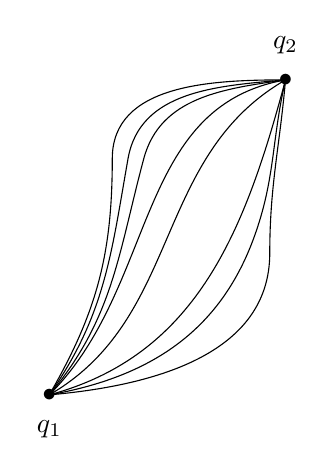
\begin{tikzpicture}
	  \node[label=below:$\bm{q}_1$]  (x1) at (6,0)  {$\bullet$};
	  \node[label=above:$\bm{q}_2$]  (x0) at (9,4)  {$\bullet$};  
	  \draw (x1.center) to [out=5,in=-90]++(2.8,1.8) to[out=90,in=-95](x0.center);
	  \draw (x1.center) to [out=10,in=-110]++(2.6,2) to[out=70,in=-103](x0.center); 
	  \draw (x1.center) to [out=15,in=-105](x0.center);
	  \draw (x1.center) to [out=30,in=-150](x0.center);
	  \draw (x1.center) to [out=45,in=-170](x0.center); 
	  \draw (x1.center) to [out=50,in=-105]++(1.2,3)to [out=75,in=-172](x0.center); 
	  \draw (x1.center) to [out=55,in=-100]++(1.0,3) to[out=80,in=-175](x0.center); 
	  \draw (x1.center) to [out=60,in=-90]++(0.8,3) to[out=90,in=-180] (x0.center);
	\end{tikzpicture}
	\caption{A graphical illustration of the possible variations with fixed endpoints $\bm{q}_{1},\bm{q}_{2}$.}
	\label{fig:variations}  
\end{figure}
